
\section{部分子分布函数}
%在粒子物理领域,主要实验工具是对撞机,并分为环形和直线,直线对撞机的质心系能量受限于加速电压和直线距离,并且没有储存环,亮度不会太高。
%所以,环形对撞机是能量前沿新物理寻找的理想工具。加速粒子种类主要有电子和质子\footnote{因为本文关注质子对撞物理,暂且不表打靶实验和其他形式对撞实验},因为电子比质子具有更强
%的同步辐射,对于同样大小的储存环,很难加速到同一能量,
质子对撞可以产生丰富的物理过程,这得益于质子是一个复合粒子。对于一定能量(GeV以上)的质子,在每次对撞中,
往往是质子的某一部分(Parton,部分子)参与相互作用(图\ref{fig:pp_collision}),
而这一部分的能量是不确定的,多种多样具有不同能量阈值的物理过程才可以发生。
但是为了准确预测各种物理过程的产生截面,我们需要了解质子中各部分子的能量分布情况。
通过深度非弹实验\cite{Kuhlen:390284},
%,单举喷注产生\cite{Aad2015-pdf}或者强子对撞机的电弱过程测量\cite{Khachatryan2016,Khachatryan2015},
我们可以得知具有特定比例动量$x$的部分子的存在概率$f(x)$,即PDF (Parton Distribution Function)。
但是这些测量均在特定$\mu$(代表散射过程中的典型能量转移大小)进行,得到的PDF须根据微扰QCD演化公式\cite{ellis_stirling_webber_1996}外推到大型强子对撞机(LHC)能量尺度。
图\ref{fig:NNPDF3}展示LHC常用的一种PDF,
值得指出的是,$\mu^2=10^4~\text{GeV}^2$表示希格斯粒子产生过程的典型能量转移,在13 TeV质心系能量下,$x$大约为$10^{-2}$,所以LHC希格斯粒子产生的主要贡献来自胶子融合。
\begin{figure}[h]
\centering
 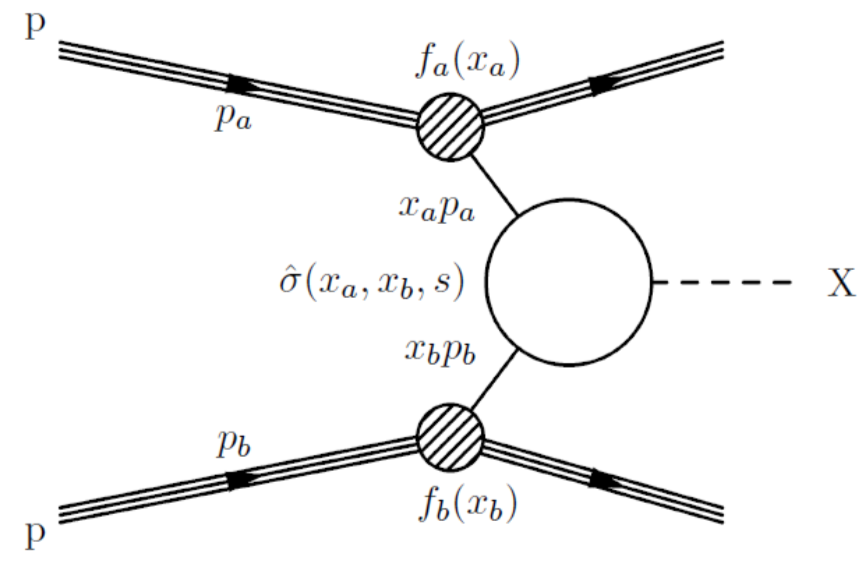
\includegraphics[width=0.75\textwidth]{fig/inclusive_pp.png}
 \caption{质子-质子对撞中的部分子硬散射过程。}
 \label{fig:pp_collision}
\end{figure}
\begin{figure}[h]
\centering
 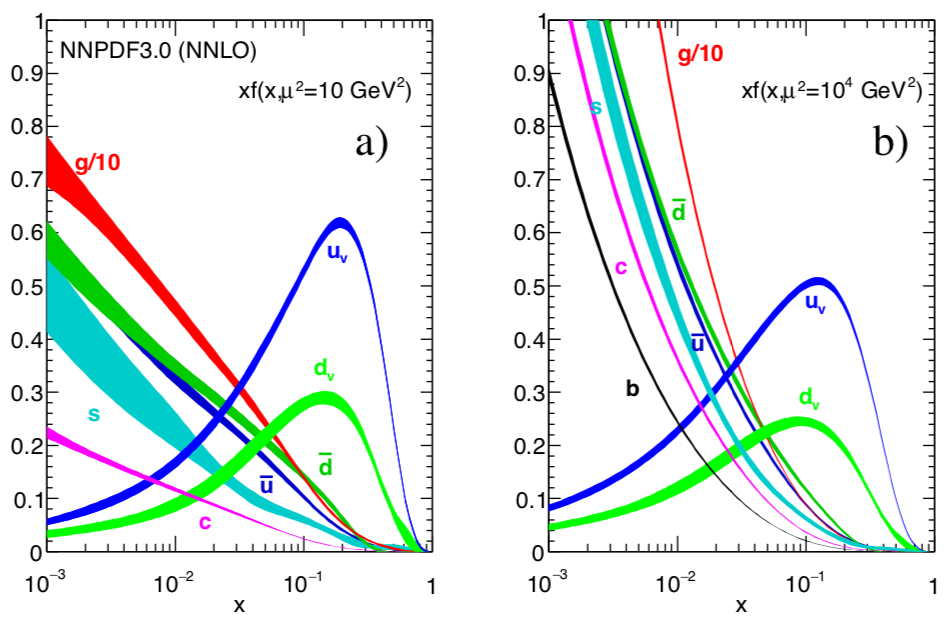
\includegraphics[width=0.75\textwidth]{fig/NNPDF3.png}
 \caption{NNPDF3.0\cite{Patrignani:2016xqp}在$\mu^2=10~\text{GeV}^2$和$\mu^2=10^4~\text{GeV}^2$时的质子部分子分布函数$xf(x)$,其中曲线宽度代表PDF误差。}
 \label{fig:NNPDF3}
\end{figure}
之后,根据因子化定理\cite{Collins:1989gx},图\ref{fig:pp_collision}所示的质子-质子对撞的单举产生截面则为:
\begin{equation}
 \sigma_{pp\rightarrow X}=\sum_{a,b}\int dx_adx_bf_a(x_a,\mu_F^2)f_b(x_b,\mu_F^2)\hat{\sigma}_{ab\rightarrow X}(x_ap_a,x_bp_b,\mu_R^2,\mu_F^2)
\end{equation}
公式中对所有可以发生某过程的各种味道部分子求和,部分子的PDF~$f_i(x_i,\mu_F^2)$依赖$\mu_F^2$,即因子化尺度,代表探查质子时的能量尺度,
而硬散射过程$ab\rightarrow X$截面还依赖于QCD重整化大小$\mu_R^2$。需要指出的是,$\mu_F$和$\mu_R$都是为了计算结果有物理意义而人为选择的参数,
在微扰QCD中,如果能够计算散射过程的所有展开阶数,物理过程的产生截面不依赖于$\mu_F$和$\mu_R$,
但是在有限阶数的计算下,$\mu_F$和$\mu_R$的大小选择会影响截面的计算结果,这也是理论误差的来源之一。
